%\fancyfood[R]{\thepage}
%\renewcommand{\headrulewidth}{0.5pt}
\chapter{General Concept and System Components  }

\chaptermark{General Concept and System Components   }
\pagestyle{fancy}
\fancyhf{}
\fancyhead[HL]{Chapter 2: General Concept and System Components}
\cfoot{\thepage}

\section{Introduction}
<<<<<<< HEAD
This chapter talks about the technical setup and the main parts used to build the IO-Box platform. It covers the hardware and software that make up the system, like the STM32G474 microcontroller,  external peripherals, sensors, tools for development, and communication protocols.

The chapter also explains the main STM32 parts used in the project, such as Analog-to-Digital Converters (ADC), Digital-to-Analog Converters (DAC), timers, and Pulse Width Modulation (PWM) features.
Knowing about these technologies is important for understanding the design and how things work, which will be explained in the next chapters.
=======
This chapter presents the technical environment and the main components used in the development of the IOBOX platform. It introduces the hardware and software resources that form the basis of the system, including the STM32G474 microcontroller, external peripherals, sensors, development tools, and communication protocols.
>>>>>>> a15e0a982f2f6d5766b8147a7f12c9c22426e956


<<<<<<< HEAD
\section{General Concept of the IO-Box Platform}
The IO-Box is a customizable industrial Input/Output system that helps connect sensors, actuators, and communication tools in IoT and automation setups.
=======
\section{General Concept of the IOBOX Platform}
The IOBOX is a configurable industrial Input/Output platform designed to facilitate the integration of sensors, actuators, and industrial communication interfaces within IoT and automation systems.
>>>>>>> a15e0a982f2f6d5766b8147a7f12c9c22426e956

It works as a bridge between field devices and control systems by gathering data from sensors, handling that data, managing external equipment, and sharing information using different communication protocols.

<<<<<<< HEAD
=======
Its modular architecture allows different hardware modules and software functionalities to be integrated according to application requirements. This flexibility makes the IOBOX suitable for a wide range of industrial monitoring, automation, and data acquisition applications.
>>>>>>> a15e0a982f2f6d5766b8147a7f12c9c22426e956

The system is built with a modular design, meaning it can include various hardware parts and software features based on what's needed for each project.
This adaptability makes it useful for many industrial tasks like monitoring, automating, and collecting data.

All these features—like strong embedded processing, multiple communication options, the ability to read both analog and digital signals, and reliable storage—are combined into one easy-to-use device.
%__Part 2 of Chapter 2: General concept and system components
\section{IOBOX Hardware architecture}
The microcontroller operates from a 3.3~V power supply and can be programmed and debugged through dedicated JTAG/SWD and UART interfaces. It provides several input and output resources, including four analog input channels connected to the ADC peripherals, seven digital input channels, seven digital output channels, and four PWM outputs for actuator control applications.

For analog signal generation, the platform integrates DAC outputs capable of producing industrial-standard 4--20~mA current signals. These outputs enable the IOBOX to interface directly with industrial control equipment and monitoring systems.

The platform supports a wide range of communication protocols to ensure compatibility with industrial and IoT environments. A USB interface is available for configuration and data exchange, while an SPI interface provides high-speed communication. Multiple I\textsuperscript{2}C buses are used for sensor integration and peripheral expansion.

Industrial communication capabilities are implemented through dedicated \linebreak transceivers. To ensure compatibility with modern industrial networks, the IOBOX integrates a TCAN330GD transceiver that enables CAN FD communication between the STM32G474 and external equipment. LIN communication is achieved through the TJA1020 LIN transceiver, while RS485 communication is implemented using the THVD1410 transceiver, enabling reliable long-distance communication and Modbus RTU integration.

To extend the number of available communication channels, the architecture incorporates a TCP9548A I\textsuperscript{2}C multiplexer, which expands a single I\textsuperscript{2}C bus into eight independent channels. Additionally, a PCF8574 I/O expander controls two CD74HC4051 multiplexers, allowing the selection of up to eight UART communication channels through a reduced number of microcontroller pins.

All interfaces are routed to dedicated external connectors, facilitating the connection of sensors, actuators, and external industrial equipment. This modular and scalable architecture provides the flexibility required for industrial automation, monitoring, data acquisition, and IoT applications while maintaining the possibility of future hardware and software extensions.

Figure~\ref{fig:synoptic_architecture} presents the overall synoptic architecture of the IOBOX platform. The system is centered around the STM32G474MBTx microcontroller, which acts as the main processing unit and coordinates data acquisition, signal processing, communication, and control functions.
\begin{figure}[H]
    \centering
    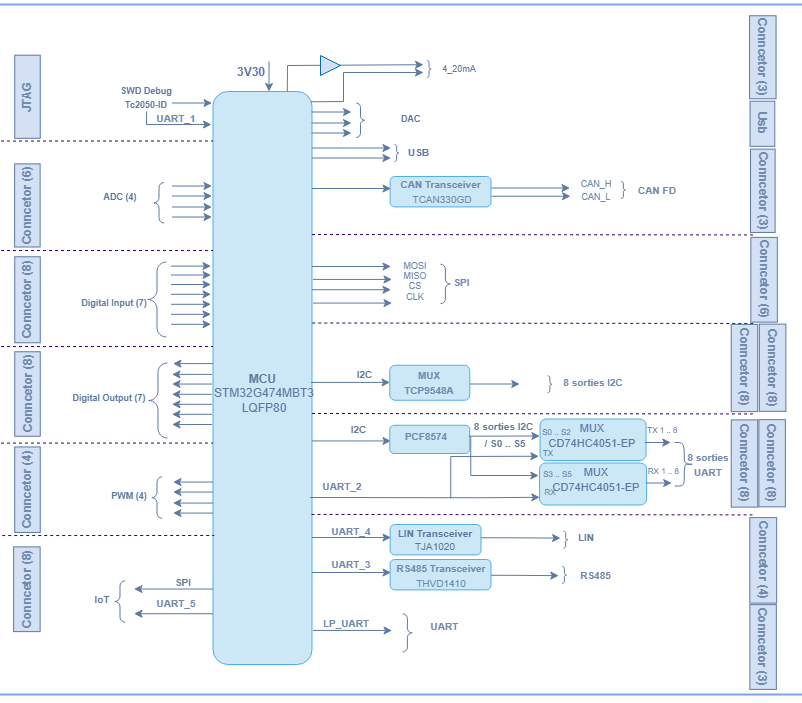
\includegraphics[width=\textwidth]{Figures/schema_synoptique.png}
    \caption{Synoptic architecture of the IOBOX platform}
    \label{fig:synoptic_architecture}
\end{figure}

\section{Hardware components}

\subsection{STM32G474MBTx Microcontroller}
At the center of the IO-Box hardware design is the STM32G474 microcontroller, a powerful chip made by STMicroelectronics. It uses the ARM Cortex-M4 processor with a floating-point unit, which makes it very good option for handling real-time signal processing and control tasks.
\begin{figure}[H]
    \centering
    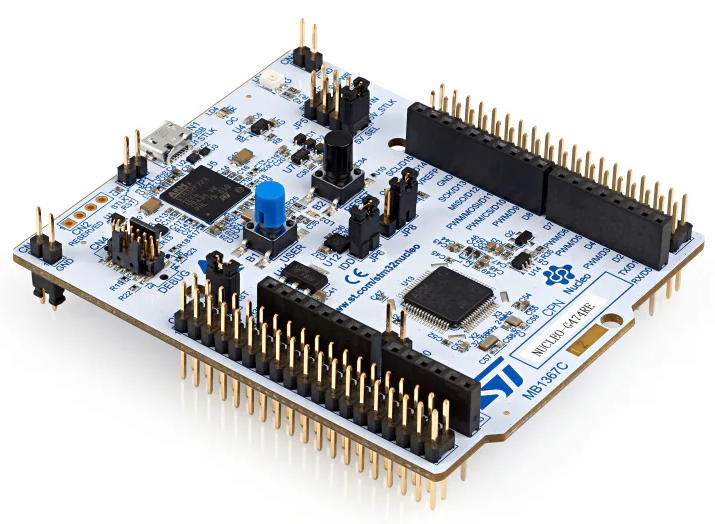
\includegraphics[width=0.55\textwidth]{Figures/nucleo-g474re.png}
    \caption{STM32G474 Microcontroller (physical package)}
    \label{fig:stm32_chip}
\end{figure}

The STM32G474 was chosen instead of the STM32F4 series because it has more ADC units (five compared to two on the F4), includes a built-in FDCAN feature, and uses a newer HAL environment. When compared to the STM32L4 series, the G474 has a faster clock speed (170 MHz versus 80 MHz) and a better analog front end, which are important for handling real-time signal processing at the needed sampling rates.

\begin{table}[H]
    \centering
    \caption{Product Attributes — STM32G474 Microcontroller}
    \label{tab:stm32g474_attributes}
    \begin{tabular}{|l|l|}
        \hline
        \textbf{Category} & Integrated Circuits, Embedded Systems, Microcontrollers \\
        \hline
        \textbf{Manufacturer} & STMicroelectronics \\
        \hline
        \textbf{Series} & STM32G4 \\
        \hline
        \textbf{Processor Core} & ARM Cortex‑M4F \\
        \hline
        \textbf{Core Size} & 32‑Bit \\
        \hline
        \textbf{Speed} & 170 MHz \\
        \hline
        \textbf{Number of I/O} & 52 \\
        \hline
        \textbf{Program Memory Size} & 512 KB Flash \\
        \hline
        \textbf{RAM Size} & 128 KB \\
        \hline
        \textbf{Data Converters} & ADC: 26 × 12‑bit; DAC: 7 × 12‑bit \\
        \hline
        \textbf{Supply Voltage} & 1.71 V – 3.6 V \\
        \hline
        \textbf{Oscillator Type} & Internal \\
        \hline
        \textbf{Operating Temperature} & –40 °C to +125 °C \\
        \hline
        \textbf{Mounting Type} & Surface Mount \\
        \hline
        \textbf{Package} & 64‑LQFP (10 × 10 mm) \\
        \hline
        \textbf{Base Product Number} & STM32G474 \\
        \hline
    \end{tabular}
\end{table}

<<<<<<< HEAD
Inside the IO-Box, the STM32G474 serves as the main processor. It handles tasks like collecting signals, processing data locally, and controlling actuators. Additionally, it manages communication with other systems using various industrial protocols, which is essential for achieving the project's goals.

\subsection{EEPROM Memory: M95M01-RDW6TP}

To manage the work with the STM32 microcontroller and make sure data is stored reliably, the IO-Box uses an external EEPROM memory called the M95M01-RDW6TP from STMicroelectronics. This device stores important information like settings, calibration data, and system logs, so the system can keep this data even when the power is turned off.
=======
Within the IOBOX, the STM32G474 acts as the central processing unit, coordinating
signal acquisition, local data processing, and actuator control. It also supervises
communication with external systems through multiple industrial protocols, making it a
key enabler of the project’s objectives.

\subsection{EEPROM Memory: M95M01-RDW6TP}

To complement the STM32 microcontroller and ensure reliable data storage, the IOBOX integrates an external EEPROM memory, specifically the M95M01‑RDW6TP from STMicroelectronics. This device provides non‑volatile storage for configuration parameters, calibration data, and system logs, allowing the platform to retain critical information even after power cycles.
>>>>>>> a15e0a982f2f6d5766b8147a7f12c9c22426e956

The M95M01-RDW6TP is a 1-Mbit serial EEPROM that is organized into 131,072 memory locations, each holding 8 bits.
It has a fast response time of 25 nanoseconds and connects through the SPI bus, which makes it easy to use with the STM32G474. It comes in an 8-pin SOIC package, making it a small and efficient option for embedded systems. It can handle up to one million write operations and keeps data safely for up to 40 years, making it a dependable choice for industrial uses where reliability is key.

\begin{table}[H]
    \centering
    \caption{Key Characteristics of M95M01‑RDW6TP EEPROM}
    \label{tab:eeprom}
    \begin{tabular}{|l|l|}
        \hline
        \textbf{Feature} & \textbf{Specification} \\
        \hline
        Manufacturer & STMicroelectronics \\
        \hline
        Type & Serial EEPROM \\
        \hline
        Capacity & 1 Mbit (131,072 × 8 bits) \\
        \hline
        Interface & SPI \\
        \hline
        Access Time & 25 ns \\
        \hline
        Package & SOIC‑8 \\
        \hline
        Endurance & 1,000,000 write cycles \\
        \hline
        Data Retention & 40 years \\
        \hline
        Operating Voltage & 1.8 V – 5.5 V \\
        \hline
    \end{tabular}
\end{table}

\begin{figure}[H]
    \centering
    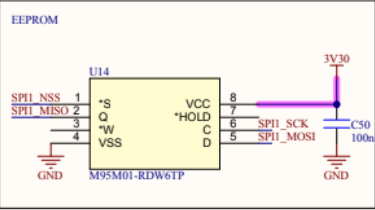
\includegraphics[width=0.5\textwidth]{Figures/eeprom.png}
    \caption{M95M01‑RDW6TP EEPROM memory chip}
    \label{fig:eeprom}
\end{figure}

\subsection{Sensors}

<<<<<<< HEAD
In the IOBox project, we added several sensors to measure different environmental and physical conditions. Our main task was to connect these sensors to the STM32G474 microcontroller, set up their settings, handle how they communicate, and do some testing to make sure the data they collect is correct. We looked closely at each sensor, learned about how they work, and wrote down their features to show how each one contributes to the whole system.
=======
In the IOBOX project, several sensors were integrated to enable environmental and physical measurements. Our work focused not only on interfacing these sensors with the STM32G474 microcontroller, but also on configuring their registers, managing communication protocols, and performing calibration to ensure accurate data acquisition. Each sensor was studied in detail, and its characteristics were documented to highlight its role within the system.
>>>>>>> a15e0a982f2f6d5766b8147a7f12c9c22426e956

\subsubsection{ENS210 Sensor}

The ENS210 is a digital sensor made by ScioSense that measures both temperature and humidity in a small size. It uses an I\textsuperscript{2}C interface to connect easily with microcontrollers like the STM32G474. The sensor is known for being accurate and using very little power, which makes it a good choice for use in systems that monitor the environment.

\begin{table}[H]
    \centering
    \caption{Key Characteristics of ENS210 Sensor}
    \label{tab:ens210}
    \begin{tabular}{|l|l|}
        \hline
        \textbf{Feature} & \textbf{Specification} \\
        \hline
        Manufacturer & ScioSense \\
        \hline
        Type & Temperature + Humidity Sensor \\
        \hline
        Interface & I\textsuperscript{2}C (16‑bit output registers) \\
        \hline
        Supply Voltage & 1.71 V – 3.6 V \\
        \hline
        Temperature Range & –40 °C to +100 °C \\
        \hline
        Temperature Accuracy & ±0.15 °C \\
        \hline
        Humidity Range & 0 – 100 \% RH \\
        \hline
       Humidity Accuracy & $\pm$2 \% RH \\
        \hline
        Package & 4‑QFN (2 × 2 mm) \\
        \hline
    \end{tabular}
\end{table}

\begin{figure}[H]
    \centering
    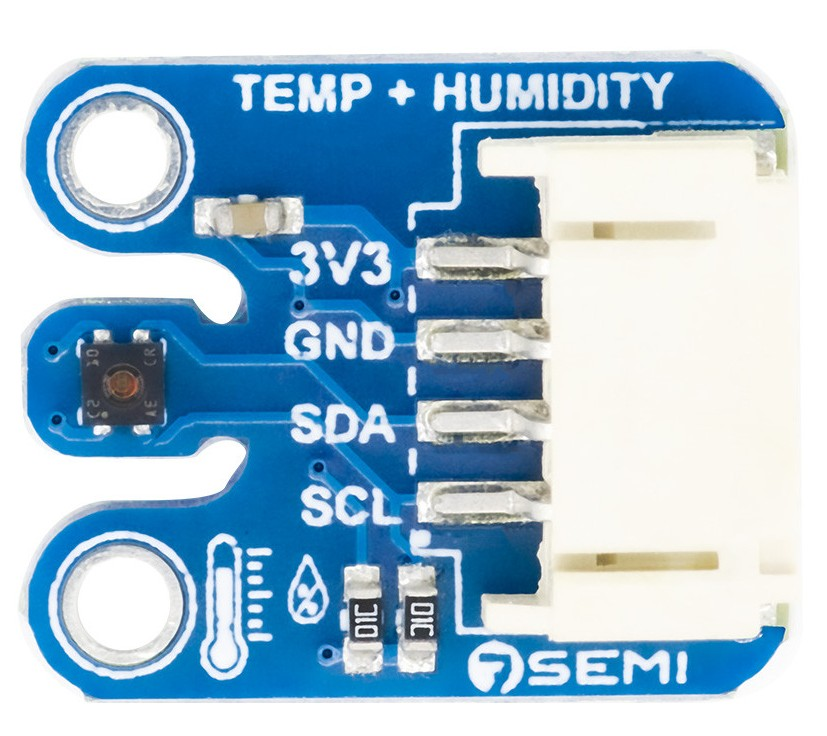
\includegraphics[width=0.3\textwidth]{Figures/ens210.jpg}
    \caption{ENS210 digital temperature and humidity sensor}
    \label{fig:ens210}
\end{figure}

\subsubsection{OPT3001DNPR Sensor}

The OPT3001DNPR is a digital light sensor made by Texas Instruments. It measures how bright the light is and shows the results in units called lux. This makes it great for uses like automatically adjusting screen brightness, controlling display backlights, and monitoring the environment. The sensor uses the I\textsuperscript{2}C communication method and has built-in calibration and a linear response over a wide range of light levels.

In the IO-Box project, the OPT3001DNPR was used to get precise light readings.
Work was done on its internal settings to set up different measurement modes, set thresholds, and run calibration processes, ensuring the sensor gave dependable data for real-time use.
\begin{table}[H]
    \centering
    \caption{Key Characteristics of OPT3001DNPR Sensor}
    \label{tab:opt3001}
    \begin{tabular}{|l|l|}
        \hline
        \textbf{Feature} & \textbf{Specification} \\
        \hline
        Manufacturer & Texas Instruments \\
        \hline
        Type & Ambient Light Sensor \\
        \hline
        Interface & I\textsuperscript{2}C \\
        \hline
        Supply Voltage & 1.6 V – 3.6 V \\
        \hline
        Measurement Range & 0.01 lux – 83,000 lux \\
        \hline
        Output Format & 16‑bit digital result in lux \\
        \hline
        Accuracy & ±10\% typical \\
        \hline
        Operating Temperature & –40 °C to +85 °C \\
        \hline
        Package & 6‑Pin WSON (2 × 2 mm) \\
        \hline
    \end{tabular}
\end{table}

\begin{figure}[H]
    \centering
    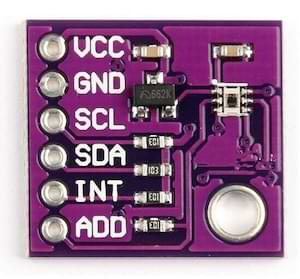
\includegraphics[width=0.3\textwidth]{Figures/opt3001.jpg}
    \caption{OPT3001DNPR ambient light sensor}
    \label{fig:opt3001}
\end{figure}

\subsubsection{HTS221TR Sensor}

The HTS221TR is a capacitive digital humidity and temperature sensor developed by STMicroelectronics. It integrates sensing elements and signal conditioning circuitry within a compact package, providing calibrated measurements through a standard I\textsuperscript{2}C interface. The sensor is designed for low-power applications while maintaining good measurement accuracy, making it suitable for environmental monitoring and industrial IoT systems.

Within the IOBOX platform, the HTS221TR is used to acquire ambient temperature and relative humidity data. Its factory-calibrated coefficients simplify integration and improve measurement reliability. Communication with the STM32G474 microcontroller is achieved through the I\textsuperscript{2}C bus, and dedicated software drivers were developed to configure the device and process sensor data.

\begin{table}[H]
    \centering
    \caption{Key Characteristics of HTS221TR Sensor}
    \label{tab:hts221}
    \begin{tabular}{|l|l|}
        \hline
        \textbf{Feature} & \textbf{Specification} \\
        \hline
        Manufacturer & STMicroelectronics \\
        \hline
        Type & Temperature + Humidity Sensor \\
        \hline
        Interface & I\textsuperscript{2}C (SPI mode not used in this project) \\
        \hline
        Supply Voltage & 1.7 V -- 3.6 V \\
        \hline
        Temperature Range & -40 °C to +120 °C \\
        \hline
        Temperature Accuracy & $\pm$0.5 °C (typ.) \\
        \hline
        Humidity Range & 0 -- 100 \% RH \\
        \hline
        Humidity Accuracy & $\pm$3.5 \% RH (typ.) \\
        \hline
        Output Resolution & 16-bit \\
        \hline
        Package & HLGA-6 (2 × 2 mm) \\
        \hline
    \end{tabular}
\end{table}

\begin{figure}[H]
    \centering
    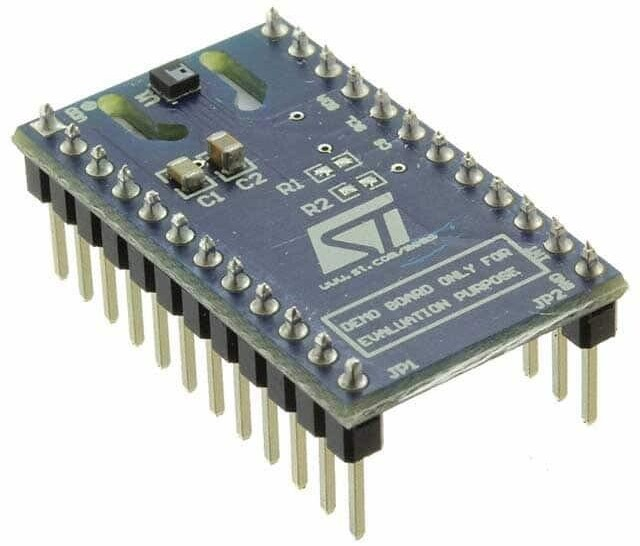
\includegraphics[width=0.3\textwidth]{Figures/hts221.jpg}
    \caption{HTS221TR temperature and humidity sensor}
    \label{fig:hts221}
\end{figure}

\section{Peripherals}

\subsection{Digital-to-Analog Converter (DAC)}
The Digital-to-Analog Converter (DAC) is an analog output peripheral integrated within the STM32G474MBTx microcontroller. It converts digital values stored in memory into continuous analog voltage levels with a resolution defined by the DAC bit width. This allows the generation of precise voltage references or analog waveforms such as sine waves, ramps, or arbitrary signals.

The DAC can operate in several modes, including software-triggered mode, timer-triggered mode, and DMA-driven mode. In timer-triggered mode, a hardware timer periodically updates the DAC output, ensuring precise and deterministic signal timing. When combined with Direct Memory Access (DMA), the DAC can continuously output precomputed waveform data without CPU intervention, significantly improving efficiency.

In the IOBox platform, the DAC is used to generate analog reference signals for actuator control. Two DAC channels are available, supporting both software-triggered and timer-triggered output modes. 

An example of DAC signal generation is illustrated in Figure~\ref{fig:dac_waveform}.

\begin{figure}[h]
\centering
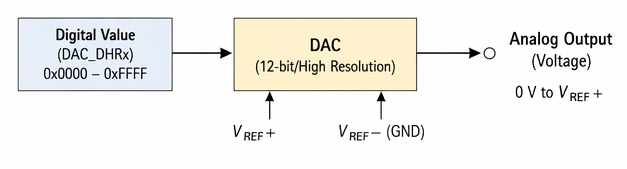
\includegraphics[width=0.65\textwidth]{Figures/dac_waveform.png}
\caption{Example of analog signal generated by DAC}
\label{fig:dac_waveform}
\end{figure}

\subsection{Analog to Digital Converter (ADC)}

The Analog‑to‑Digital Converter (ADC) is a fundamental peripheral in embedded systems, responsible for transforming continuous analog signals into discrete digital values that can be processed by the microcontroller. This conversion is essential for applications where physical phenomena such as temperature, pressure, or current must be measured and interpreted by digital logic.

In the IOBox project, ADCs are employed to acquire signals from sensors and external modules, enabling precise monitoring and control. The STM32G474 microcontroller integrates multiple high‑resolution ADC channels, allowing simultaneous sampling of different inputs. This capability is particularly important in industrial contexts where multiple signals must be captured in real time.

The operation of an ADC follows a well‑defined process. The analog input is sampled at regular intervals determined by the sampling frequency. Each sample is then quantized into a digital value according to the converter’s resolution (e.g., 12‑bit or 16‑bit). The resulting digital word represents the amplitude of the analog signal at that instant. The accuracy of this conversion depends on factors such as resolution, sampling rate, and reference voltage stability.

Key characteristics of ADCs include:
\begin{itemize}
    \item \textbf{Resolution}: Defines the number of discrete levels available.
    \item \textbf{Sampling Rate}: Determines how frequently the analog signal is measured, affecting the fidelity of dynamic signals.
    \item \textbf{Reference Voltage}: Sets the maximum measurable input range, ensuring proper scaling of the digital output.
    \item \textbf{Input Channels}: Multiple channels allow acquisition from several sensors simultaneously.
    \item \textbf{Conversion Modes}: Support for single, continuous, and DMA‑driven conversions, enabling flexible integration into firmware.
\end{itemize}

Within the IO‑Box, ADCs are used to capture sensor data such as voltage levels, current measurements, or other analog signals. These values are then processed by the firmware to generate meaningful information, trigger control actions, or communicate results to external supervisory systems.

\begin{figure}[H]
    \centering
    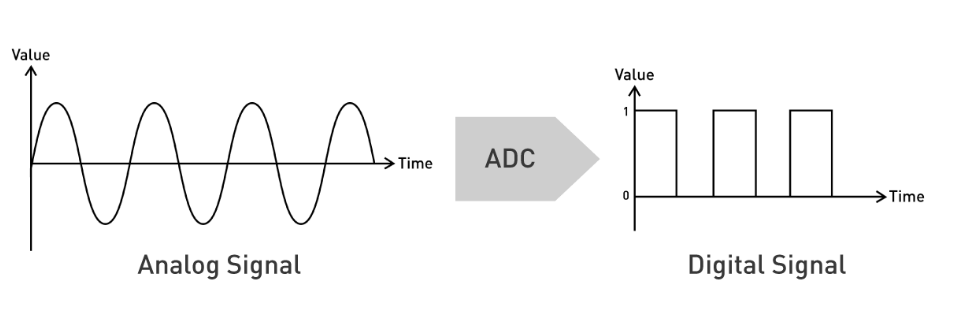
\includegraphics[width=0.70\textwidth]{Figures/ADC.png}
    \caption{Basic ADC conversion from analog input to digital output}
    \label{fig:adc}
\end{figure}

\subsection{Timers}

Timers are fundamental peripherals in the STM32G474 microcontroller, designed to provide accurate time base generation, event counting, and signal measurement. They operate by incrementing or decrementing a counter register according to a clock source, and can trigger actions when predefined values are reached.

Key functionalities of timers include:
\begin{itemize}
    \item \textbf{Time Base Generation}: Creating precise delays or periodic events.
    \item \textbf{Input Capture}: Measuring external signal characteristics such as frequency or pulse width.
    \item \textbf{Output Compare}: Generating events when the counter matches a reference value.
    \item \textbf{Synchronization}: Coordinating multiple timers for complex control tasks.
    \item \textbf{Advanced Features}: Dead‑time insertion, break inputs, and complementary outputs for safe power electronics control.
\end{itemize}

Timers are essential for scheduling tasks, measuring sensor signals, and driving peripherals that require precise timing.


\subsection{Pulse Width Modulation (PWM)}

Pulse Width Modulation (PWM) is a technique used to encode analog information into a digital waveform by varying the duty cycle of a periodic signal. In embedded systems, PWM is widely used for motor control, LED dimming, and power regulation.

PWM signals in the STM32G474 are generated using timers. The timer counts up to a predefined value stored in the auto‑reload register (ARR), while the compare register (CCR) defines the switching point of the output. The ratio between the high time and the total period represents the duty cycle. By adjusting ARR and CCR, both frequency and duty cycle can be controlled with high precision.

Key characteristics of PWM include:
\begin{itemize}
    \item \textbf{Frequency}: Determined by prescaler and ARR configuration.
    \item \textbf{Duty Cycle}: Defined by CCR relative to ARR.
    \item \textbf{Resolution}: Limited by timer bit width (typically 16‑bit).
    \item \textbf{Complementary Outputs}: Enable safe control of MOSFET drivers in half‑bridge or full‑bridge circuits.
    \item \textbf{Applications}: Motor drivers, LED dimming, switching converters, and DAC emulation.
\end{itemize}

\begin{figure}[H]
    \centering
    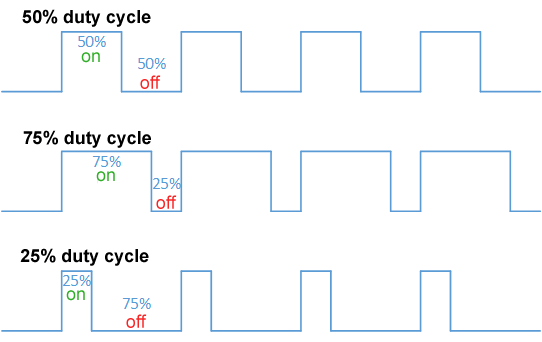
\includegraphics[width=0.6\textwidth]{Figures/Duty_Cycle_Examples.png}
    \caption{Illustration of PWM signals with different duty cycles}
    \label{fig:pwm}
\end{figure}

\section{Communication Protocols}

\subsection{I2C Protocol}
Inter-Integrated Circuit (I2C) is a synchronous, half-duplex serial communication protocol widely used for communication between integrated circuits over short distances. It relies on two bidirectional lines: the Serial Data Line (SDA) and the Serial Clock Line (SCL), both requiring pull-up resistors. The protocol follows a master-slave architecture, where the master initiates communication and generates the clock signal.

Each device connected to the bus is identified by a unique address. Data is then exchanged one byte at a time, with each byte followed by an acknowledgment bit (ACK/NACK) from the receiving device. The communication is terminated by a STOP condition. I2C supports different speed modes, including Standard Mode (100 kHz), Fast Mode (400 kHz), and higher-speed variants.

The I2C frame structure is illustrated in Figure~\ref{fig:i2c_frame}.

\begin{figure}[h]
\centering
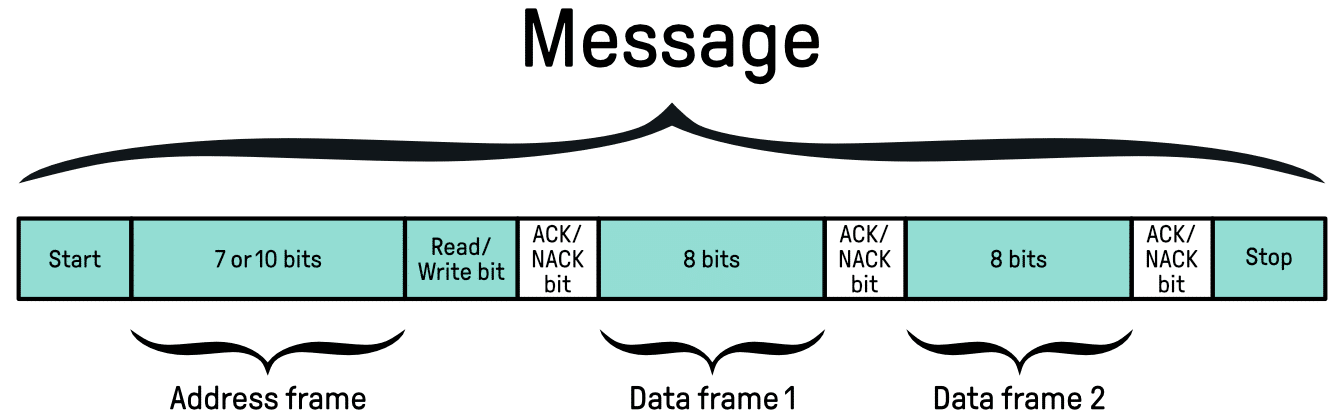
\includegraphics[width=0.7\textwidth]{Figures/i2c_frame.png}
\caption{I2C frame format}
\label{fig:i2c_frame}
\end{figure}

In this project, the I2C interface of the STM32G474MBTx is configured using the HAL library generated by STM32CubeMX. It is used to communicate with external peripherals such as sensors and low-speed devices. The implementation relies on interrupt or polling-based data transfers depending on timing constraints. Particular attention is given to bus stability, including proper pull-up resistor sizing and handling of potential communication errors such as bus busy states or missing acknowledgments.

As shown in Figure~\ref{fig:i2c_bus}, the I2C bus allows multiple slave devices.

\begin{figure}[h]
\centering
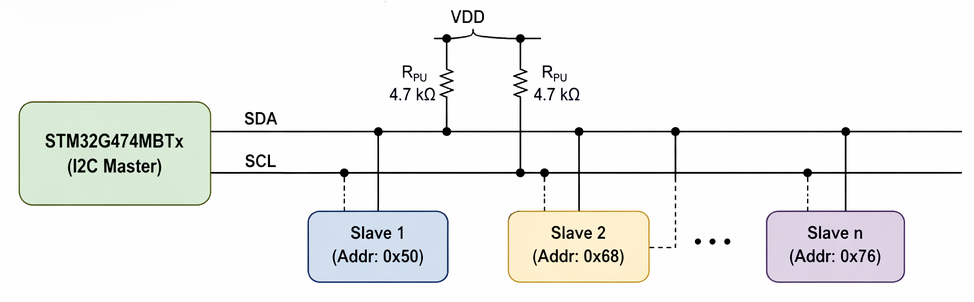
\includegraphics[width=0.7\textwidth]{Figures/i2c_bus.png}
\caption{I2C communication bus architecture}
\label{fig:i2c_bus}
\end{figure}

\subsection{Serial Peripheral Interface (SPI)}

The Serial Peripheral Interface (SPI) is a synchronous serial communication protocol widely used in embedded systems. It enables high‑speed data exchange between a microcontroller and peripheral devices such as sensors, memory modules, or communication transceivers. SPI operates in a master–slave configuration, where the microcontroller typically acts as the master, controlling the clock and data flow.

In the IOBOX project, SPI is employed to ensure reliable and efficient communication with external modules that require fast data transfer. Its simplicity and speed make it suitable for real‑time applications, particularly when multiple peripherals must be interfaced with the STM32 microcontroller.

SPI communication is based on a clock signal generated by the master device. Each bit of data is shifted out on the MOSI line while simultaneously another bit is shifted in on the MISO line. This process is synchronized by the clock (SCLK), ensuring deterministic timing. The communication sequence typically follows these steps: the master activates the Chip Select (CS) line of the desired slave, provides the clock signal, transmits data bit‑by‑bit on MOSI while receiving data on MISO, samples the data according to the configured mode, and finally deactivates the CS line to end the session. This mechanism allows full‑duplex communication, meaning data can be transmitted and received simultaneously.

SPI supports four modes of operation (Mode 0 to Mode 3), determined by the configuration of clock polarity (CPOL) and clock phase (CPHA). This flexibility ensures compatibility with a wide range of peripheral devices. Key characteristics of SPI include its high speed (operating at several MHz), simple wiring with four main signals (MOSI, MISO, SCLK, CS), and scalability through multiple slave connections.

\begin{figure}[H]
    \centering
    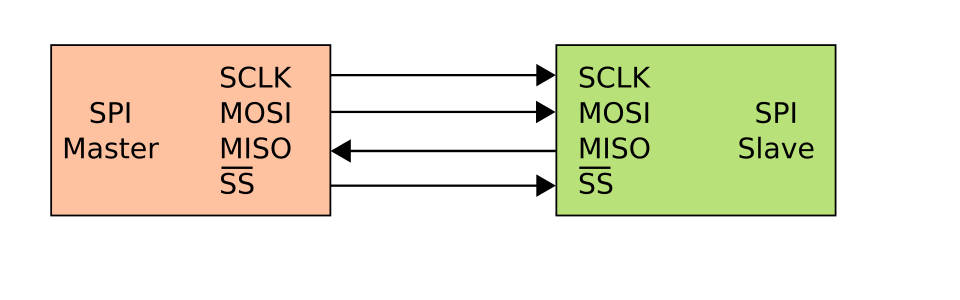
\includegraphics[width=0.65\textwidth]{Figures/spi_diagram.png}
    \caption{Basic SPI communication between master and slave devices}
    \label{fig:spi}
\end{figure}

\subsection{UART Protocol}
Universal Asynchronous Receiver-Transmitter (UART) is an asynchronous serial communication protocol that enables full-duplex data exchange between devices without a shared clock signal. Data is transmitted over two lines: Transmit (TX) and Receive (RX). Synchronization between devices is achieved by configuring identical communication parameters, including baud rate, data bits, parity, and stop bits.

Each data frame typically consists of a start bit, followed by a configurable number of data bits (usually 8), an optional parity bit for error detection, and one or more stop bits. Unlike synchronous protocols, UART does not include a clock line, making it simpler but more sensitive to timing mismatches.

In this project, UART is used for communication between the STM32 microcontroller and external systems such as a host computer or other embedded modules. It plays a key role in debugging, logging, and real-time data exchange. The implementation uses the STM32 HAL drivers with support for interrupt-driven and DMA-based transmission to ensure efficient and non-blocking communication. Error handling mechanisms, including overrun, framing, and noise errors, are also considered to improve communication reliability.

The UART frame structure is illustrated in Figure~\ref{fig:uart_frame}.

\begin{figure}[h]
\centering
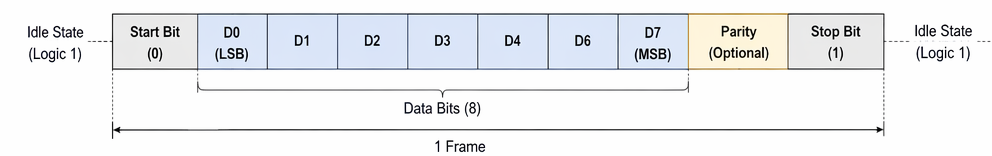
\includegraphics[width=0.9\textwidth]{Figures/uart_frame.png}
\caption{UART frame format}
\label{fig:uart_frame}
\end{figure}


\subsection{RS485 Communication}
RS485 is a robust differential serial communication standard widely used in industrial environments due to its high noise immunity and long-distance capabilities. Unlike single-ended UART communication, RS485 transmits data over a differential pair of lines (A and B), where the information is encoded as a voltage difference between the two conductors. This approach significantly reduces susceptibility to electromagnetic interference and ground potential differences.

The RS485 standard supports half-duplex communication in multi-drop configurations, allowing multiple nodes to share the same bus. However, only one device can transmit at a time, which requires proper bus arbitration at the software level or through protocol design.

In this project, RS485 serves as the physical layer for Modbus RTU communication. A dedicated UART peripheral (USART3) is used with an external RS485 transceiver to convert TTL logic levels to differential signals. Direction control is managed in software, as described in Chapter 3.

Before transmission, the microcontroller sets the DE pin high to enable the driver stage. After sending the data frame, the DE pin is reset to return the transceiver to reception mode. This timing control is critical to avoid bus contention. The communication is typically used for reliable data exchange in noisy environments, especially when longer cable lengths are required compared to standard UART.

Figure~\ref{fig:rs485_bus} illustrates a typical RS485 bus configuration.

\begin{figure}[h]
    \centering
    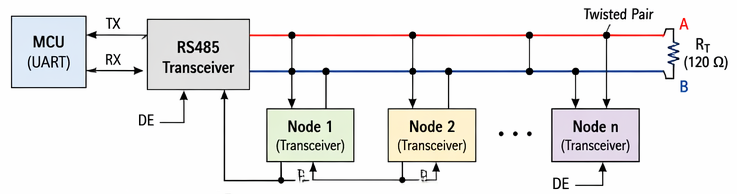
\includegraphics[width=0.65\textwidth]{Figures/rs485_bus.png}
    \caption{RS485 differential bus with multi-node configuration}
    \label{fig:rs485_bus}
\end{figure}

\subsection{Modbus Protocol}

Modbus is one of the most widely used industrial communication protocols for exchanging data between electronic devices. Originally developed by Modicon in 1979, it follows a client-server (master-slave) architecture and enables communication between programmable logic controllers (PLCs), sensors, actuators, Human-Machine Interfaces (HMIs), and embedded systems.

Modbus defines a standardized message structure that allows devices from different manufacturers to communicate using a common protocol. Two main variants are commonly used: Modbus RTU, which operates over serial communication interfaces such as RS232 and RS485, and Modbus TCP, which operates over Ethernet networks.

In the IOBOX project, Modbus RTU is implemented over the RS485 physical layer to ensure reliable communication in industrial environments. The STM32G474 microcontroller acts as either a Modbus master or slave depending on the application requirements. Through Modbus registers, external systems can access sensor measurements, configuration parameters, status information, and control commands.

In this project, the IOBox operates as a Modbus RTU slave at address 0x01, communicating over RS485 at 19,200 bps. The slave implementation supports function codes FC01 through FC06, FC15, and FC16. Input registers expose real-time sensor measurements (temperature, humidity, illuminance) to any connected Modbus master, and holding registers allow actuator control. The implementation details are described in Chapter 3.

A Modbus RTU frame consists of four main fields:

\begin{itemize}
    \item \textbf{Slave Address}: Identifies the target device.
    \item \textbf{Function Code}: Specifies the requested operation.
    \item \textbf{Data Field}: Contains transmitted data or register information.
    \item \textbf{CRC Field}: Provides error detection for frame integrity.
\end{itemize}

\begin{figure}[H]
    \centering
    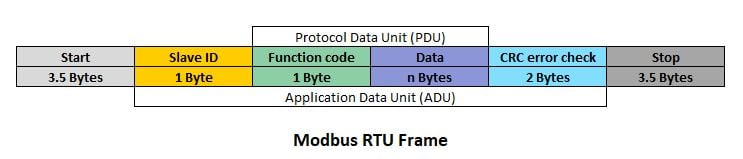
\includegraphics[width=0.8\textwidth]{Figures/modbus_rtu_frame.jpg}
    \caption{Typical Modbus RTU frame structure}
    \label{fig:modbus_frame}
\end{figure}

To ensure compatibility with standard industrial devices, the implementation supports a subset of Modbus function codes, classified according to their role in data access and control:

\begin{table}[H]
    \centering
    \caption{Supported Modbus Function Codes in the IOBOX Platform}
    \label{tab:modbus_function_codes}
    \begin{tabular}{|c|c|p{7cm}|}
    \hline
    \textbf{Function Code} & \textbf{Name} & \textbf{Description} \\
    \hline
    FC01 & Read Coils & Reads digital output states (ON/OFF status) \\
    \hline
    FC02 & Read Discrete Inputs & Reads digital input signals from sensors or switches \\
    \hline
    FC03 & Read Holding Registers & Reads configuration and control registers (16-bit) \\
    \hline
    FC04 & Read Input Registers & Reads real-time measurement data (sensor values) \\
    \hline
    FC05 & Write Single Coil & Controls a single digital output (ON/OFF command) \\
    \hline
    FC06 & Write Single Register & Writes a single 16-bit configuration or control value \\
    \hline
    FC15 & Write Multiple Coils & Updates multiple digital outputs in one request \\
    \hline
    FC16 & Write Multiple Registers & Writes multiple registers for bulk configuration/control \\
    \hline
    \end{tabular}
\end{table}

This classification enables structured interaction with the IOBOX memory map, separating real-time acquisition data (input registers) from controllable parameters (holding registers). It also ensures interoperability with a wide range of Modbus-compatible supervisory systems such as SCADA platforms and PLCs.

\subsection{Controller Area Network (CAN)}

The Controller Area Network (CAN) is a robust serial communication protocol originally developed for automotive applications, but now widely used in industrial and embedded systems. It enables reliable data exchange between multiple devices without requiring a central host, making it ideal for distributed control systems.

In the IOBOX project, CAN is employed to ensure communication with industrial equipment and sensors that demand high reliability and fault tolerance. Its ability to handle multiple nodes on a single bus makes it particularly suitable for environments where numerous devices must share information in real time.

CAN communication is based on a message‑oriented protocol. Instead of addressing specific devices directly, each message carries an identifier that defines its priority and content. This allows multiple nodes to listen simultaneously and decide whether to act on the received data. The arbitration mechanism ensures that when two nodes attempt to transmit at the same time, the message with the highest priority (lowest identifier value) wins, while the other node waits until the bus is free. This guarantees deterministic communication without collisions.

Key characteristics of CAN include:
\begin{itemize}
    \item \textbf{Multi‑master capability}: Any node can initiate communication when the bus is idle.
    \item \textbf{Error detection and handling}: Built‑in mechanisms such as CRC checks, acknowledgment bits, and error frames ensure data integrity.
    \item \textbf{Priority‑based arbitration}: Messages are prioritized by identifiers, ensuring that critical data is transmitted first.
    \item \textbf{Scalability}: Supports up to 112 nodes on a single bus, making it suitable for complex systems.
    \item \textbf{Speed}: Operates up to 1 Mbps in classical CAN, and higher in CAN FD (Flexible Data‑Rate), which extends payload size and transmission speed.
\end{itemize}

\begin{figure}[H]
    \centering
    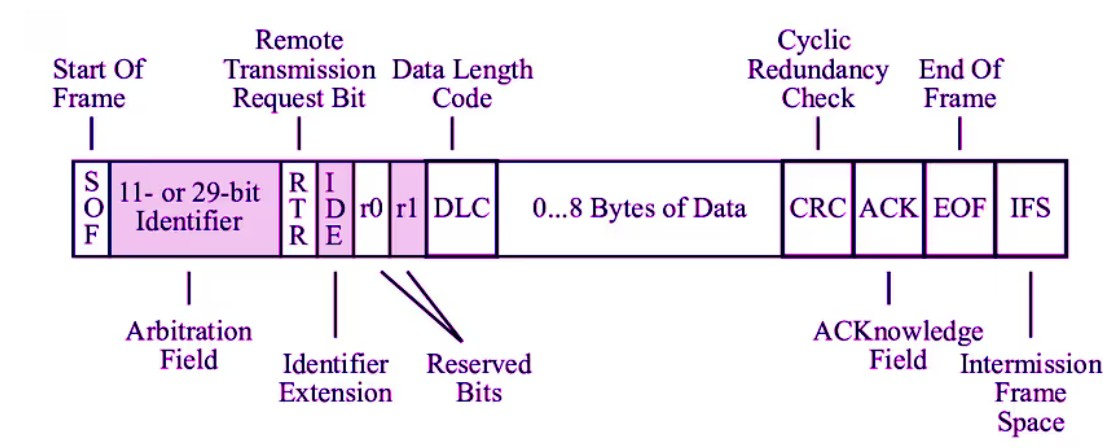
\includegraphics[width=0.70\textwidth]{Figures/trame_can.jpg}
    \caption{Basic CAN frame}
    \label{fig:can_frame}
\end{figure}

In practice, CAN uses two differential lines, CAN\_H and CAN\_L, to transmit data. This differential signaling improves noise immunity and allows reliable communication even in electrically harsh environments. Each frame consists of fields such as the start of frame, identifier, control bits, data payload, CRC, and end of frame, ensuring structured and error‑resistant communication.

\begin{figure}[H]
    \centering
    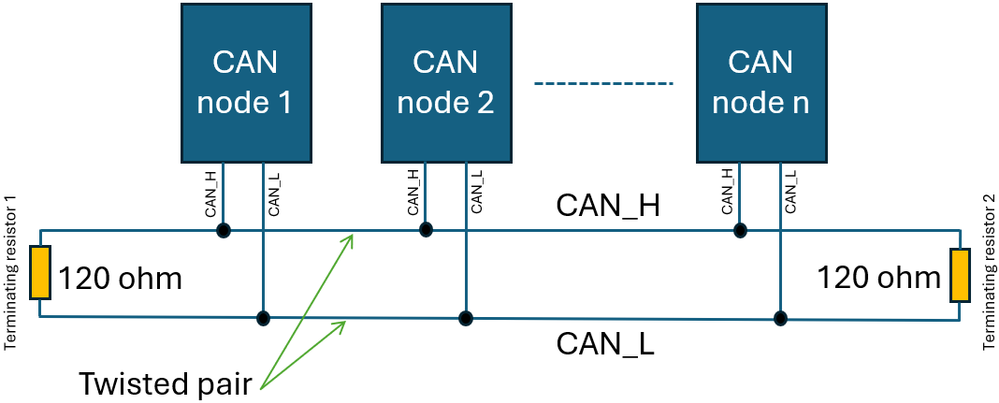
\includegraphics[width=0.70\textwidth]{Figures/can_diagram.png}
    \caption{Basic CAN bus communication with multiple nodes}
    \label{fig:can_bus}
\end{figure}

\subsection{LIN Protocol}
\nobreak{}
Local Interconnect Network (LIN) is a low-cost serial communication protocol designed for distributed control systems, particularly in automotive applications. It operates on a single-wire physical layer and follows a strict master-slave architecture where the master node controls the entire bus communication schedule.

Unlike event-driven protocols, LIN is time-triggered, meaning communication is organized into predefined frames sent at fixed intervals. Each frame consists of a header transmitted by the master and a response transmitted by a slave node. The header includes a break field (used to signal the start of a frame), a synchronization byte, and an identifier field that determines which node should respond.

The data response typically contains up to 8 bytes, followed by a checksum used for error detection. LIN achieves deterministic timing by enforcing strict scheduling, making it suitable for non-critical but predictable control tasks.

In this project, LIN communication is implemented using the STM32 UART peripheral configured in LIN mode. The hardware support simplifies break detection and synchronization field handling, reducing software complexity. The system can therefore reliably detect frame boundaries and process incoming data with minimal CPU overhead.

The LIN frame structure is shown in Figure~\ref{fig:lin_frame}.

\begin{figure}[h]
\centering
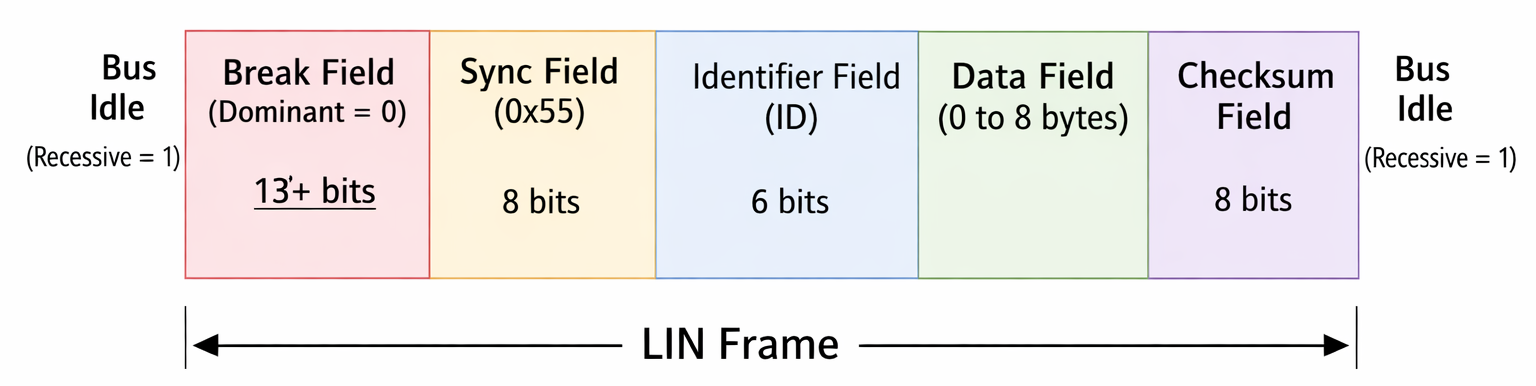
\includegraphics[width=0.8\textwidth]{Figures/lin_frame.png}
\caption{LIN frame structure}
\label{fig:lin_frame}
\end{figure}

\section{Software tools}

\subsection{Visual Studio Code}
Visual Studio Code (VS Code) is a lightweight yet powerful source code editor optimized for modern software development. It supports multiple programming languages and provides advanced features such as syntax highlighting, intelligent code completion, and debugging tools. 

In this project, Visual Studio Code was used as the primary text editor for documentation, script editing, and Git-based version control. Extensions such as Git Graph enabled visualization of commit history, branch management, and tracking of code evolution across the development team.

\begin{figure}[H]
    \centering
    
\includegraphics[width=0.2\textwidth]{Figures/vs_code.jpeg}
    \caption{Visual Studio Code interface}
    \label{fig:vscode}
\end{figure}

\subsection{IAR Embedded Workbench}
IAR Embedded Workbench (IAR EW) is a professional integrated development environment (IDE) dedicated to embedded systems programming, particularly for microcontrollers such as the STM32 family. It provides a highly optimized C/C++ compiler, advanced debugging capabilities, and efficient project management tools. 

In this project, IAR EW was used for firmware development, compilation, and debugging. Its powerful optimization features contributed to generating efficient and reliable embedded code, which is critical for real-time applications and resource-constrained systems\cite{21}.

\begin{figure}[H]
    \centering
    
\includegraphics[width=0.2\textwidth]{Figures/iar_workbench.png}
    \caption{IAR Embedded Workbench IDE}
    \label{fig:iar}
\end{figure}

\subsection{STM32CubeMX}
STM32CubeMX is a graphical configuration tool developed by STMicroelectronics for STM32 microcontrollers. It allows developers to easily configure peripherals, clock settings, and pin assignments through an intuitive interface. The tool also generates initialization code based on the selected configuration, significantly reducing development time and minimizing configuration errors. 

In this project, STM32CubeMX was used in a limited capacity: it was invoked once at the beginning of the project to generate the initial project skeleton, configure the system clock (HSI PLL at 170 MHz), and enable the Serial Wire Debug interface. The peripheral initialization functions that CubeMX would normally generate were intentionally not used. Instead, all peripheral drivers were developed as handwritten BSP (Board Support Package) modules, which are described in detail in Chapter 3. CubeMX thus served exclusively as a project scaffolding and clock configuration tool.

\begin{figure}[H]
    \centering
    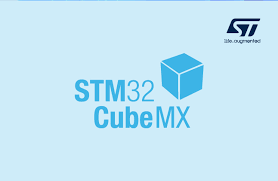
\includegraphics[width=0.4\textwidth]{Figures/stm32cubemx.png}
    \caption{STM32CubeMX configuration interface}
    \label{fig:cubemx}
\end{figure}

\subsection{GitLab}

GitLab was used as the version control and collaboration platform throughout the project. The repository was organized by module (BSP, Managers, Application), with branches used to isolate feature development and avoid conflicts during parallel work. Commit history served as a development log, and merge requests were used to review code before integrating changes into the main branch.

\begin{figure}[H]
    \centering
    
\includegraphics[width=0.2\textwidth]{Figures/gitlab_logo.png}
    \caption{GitLab logo}
    \label{fig:gitlab}
\end{figure}

\subsection{Conclusion}

In this chapter, we presented the general concept and system components of the IO‑Box project. We began with the synoptic diagram, which outlined the main functional phases of acquisition, filtering, regulation, and transmission/actuation. We then introduced the software architecture, organized into four distinct layers (HAL, BSP, Manager, and Application), and complemented this with the hardware architecture, highlighting the STM32G474 microcontroller, power supply design, communication interfaces, and peripheral modules. Finally, we described the development tools and protocols that support the implementation of the system.

By establishing this technical foundation, Chapter 3 has clarified the resources and methodologies that will be employed in the realization phase. The next chapter will be dedicated to the practical implementation of the IO‑Box, detailing the firmware design, register configuration, BSP development, and integration of sensors and actuators into a coherent and functional platform.